\documentclass[]{article}

%opening
\usepackage{graphbox}	% permette di modificare i margini
\usepackage{graphicx}
\usepackage{float}
\usepackage{longtable}
\usepackage{array}
\usepackage{fancyhdr}
\pagestyle{fancy}

\newcommand{\copertina}{
	\begin{titlepage}
		\begin{center}
			
			
\includegraphics[width=0.4\linewidth]{graphics/icon2.png}\\
			\vspace{1cm}
			
			\begin{Huge}
				\textbf{Centro Estetico Nirvana} \\
			\end{Huge}
			
			\vspace{9pt}  
			
			\begin{large}
				\textbf{Progetto per il corso di Tecnologie Web\\}
				\textbf{A.A.} 2022/2023\\
				\vspace{3pt}
			\end{large}	  
			
			\vspace{24pt}
			
			\begin{large}
				\textbf{Indirizzo sito web:} \href{http://tecweb.studenti.math.unipd.it/nbaesso}{http://tecweb.studenti.math.unipd.it/nbaesso}\\
			\end{large} 
			
			\vspace{10pt} 
			
			\bgroup
			\def\arraystretch{1.3}
			\centering
			\begin{tabular}{r|L{5cm}}
			\multicolumn{2}{c}{\textbf{Informazioni sul gruppo} } \\ \hline
			\textbf{Membri} &  Nicola Baesso - 2011877 \newline Matteo Cusin - 2008073 \newline Annalisa Egidi - 1216745 \newline Lisien Skenderi - 2023461\\
			\end{tabular}
			\egroup
			
			\begin{center}
				\textbf{Referente\\}
				Nicola Baesso - nicola.baesso@studenti.unipd.it\\
				\textbf{Utenti (credenziali username-password):\\}
				\textit{Amministratore:} admin - admin\\
				\textit{Cliente:} user - user\\
			\end{center}
			
		\end{center}
	\end{titlepage}
}	%FINE NEW COMMAND COPERTINA

\usepackage{lastpage}
\usepackage{fancyhdr}
\fancypagestyle{plain}{
	% cancella tutti i campi di intestazione e piè di pagina
	\fancyhf{}
	
	\lhead{
		
\includegraphics[width=0.1\linewidth]{graphics/icon2.png}
	}
		\rhead{
		Centro Estetico Nirvana
	}

	\lfoot{ %piè di pagina a sx
		Relazione Progetto Tecnologie Web
	}
	\rfoot{Pagina \thepage{} di \pageref{LastPage}} %es: pag: 4 di 10
	
	%linea orizzontale alle posizioni top e bottom della pagina (se è 0, non c'è la linea)
	\renewcommand{\headrulewidth}{0.3pt}  
	\renewcommand{\footrulewidth}{0.3pt}
}
\pagestyle{plain}

%\usepackage{calc} %introduce la notazione infissa per le op. aritmetiche interne a LaTeX

\usepackage[utf8]{inputenc}
%\usepackage{cm-super}

\usepackage{lmodern}
\usepackage[T1]{fontenc}
\usepackage[italian]{babel} %il documento è in italiano
%\usepackage{textcomp} %The pack­age sup­ports the Text Com­pan­ion fonts, which pro­vide many text sym­bols
%(such as baht, bul­let, copy­right, mu­si­cal­note, onequar­ter, sec­tion, and yen), in the TS1 en­cod­ing.

\usepackage{graphicx}       %permette di inserire delle immagini
\usepackage{caption}        %numerazione figure e loro descrizione testuale
\usepackage{subcaption}     %sottofigure numerabili
\usepackage{float}  %permette di inserire un # qualsiasi di figure fluttuanti
\usepackage[dvipsnames,table]{xcolor}
\usepackage{rotating} %permette di ruotare le immagini
%\usepackage{changepage} %utile se c'è bisogno di aggiustare margini per centrare figure

\usepackage{listings} %permette di inserire degli spezzoni di codice

\usepackage{tikz} %disegno di immagini vettoriali a schermo. Utile per grafi
\usetikzlibrary{arrows.meta}
\usetikzlibrary{graphs}
\usetikzlibrary{arrows}
%\usepackage{tikz-uml} %serve per disgnare l'UML, fantastica guida:
%https://perso.ensta-paristech.fr/~kielbasi/tikzuml/var/files/doc/tikzumlmanual.pdf
%download package: http://perso.ensta-paristech.fr/~kielbasi/tikzuml/

%package per le tabelle
\usepackage{booktabs} %permette di poter usare delle liste nelle tabelle
\usepackage{tabularx} 
\usepackage{longtable} %una tabella può continuare su più pagine
\usepackage{multirow} %utile per visualizzare una cella su più righe
%\usepackage{multicolumn} %cella su più colonne
%\usepackage[table]{xcolor} %rende disponibile l'utilizzo di un colore per lo sfondo
%delle celle di una tabella

%crea una cella per le tabelle in grado di andare a capo con \newline
%https://tex.stackexchange.com/questions/12703/how-to-create-fixed-width-table-columns-with-text-raggedright-centered-raggedlef
\usepackage{array}
\newcolumntype{L}[1]{>{\raggedright\let\newline\\\arraybackslash\hspace{0pt}}m{#1}}
\newcolumntype{C}[1]{>{\centering\let\newline\\\arraybackslash\hspace{0pt}}m{#1}}
\newcolumntype{R}[1]{>{\raggedleft\let\newline\\\arraybackslash\hspace{0pt}}m{#1}}


%indice con i puntini
\usepackage{tocloft}
\renewcommand\cftsecleader{\cftdotfill{\cftdotsep}}

%http://ctan.mirror.garr.it/mirrors/CTAN/macros/latex/contrib/appendix/appendix.pdf
\usepackage{appendix} %aggiunge dei comandi per l'appendice
\usepackage{parskip} %aiuta LaTeX a trovare il miglior stile per i page break
\setcounter{secnumdepth}{5} % numera i sottoparagrafi
\setcounter{tocdepth}{5} %aggiunge all'indice i sottoparagrafi
%\usepackage{titlesec} %\begin{paragraph} si può usare come subsubsubsection!

\usepackage{breakurl}%\url{...} può continare alla linea successiva. (si può andare a capo)

\usepackage[colorlinks=true]{hyperref}
\hypersetup{
	colorlinks=true,
	citecolor=black,
	filecolor=black,
	linkcolor=black, % colore dei link interni
	urlcolor=Maroon  % colore dei link interniesterni
}

%per alcune liste, permette di usare 'alligator' nei labeling 
\usepackage{blindtext} 
\usepackage{scrextend} 
\addtokomafont{labelinglabel} 
{\sffamily}

%FILE INCLUSI
\usepackage{graphicx}

\begin{document}

\copertina
\tableofcontents
\newpage
\section{Introduzione}
Il centro estetico Nirvana vuole implementare un sito Internet al fine di poter fornire informazioni riguardo al centro stesso.\\
Il sito dovrà contenere informazioni riguardo i trattamenti disponibili e i macchinari utilizzati per essi, nonchè informazioni sulle consulenze e ogni informazione relativa a dove si trova il centro e quali orari di apertura osserva.\\
Inoltre, permette agli utenti di richiedere una consulenza o un trattamento, che necessita di essere confermato o meno dal centro stesso. Le prenotazioni possono anche inserite, oltre che confermate o smentite, anche dal centro stesso.\\
É fondamentale che il sito garantisca accessibilitá, in modo da permettere a chiunque di poter essere utilizzato, e usabilitá, separando struttura, presentazione e comportamento.\\
Si vuole infine garantire una navigazione fluida tra i contenuti del sito, evitando al piú possibile il disorientamento e prevedendo il giusto supporto per ritornare all'interno del sito stesso.\\
\section{Analisi}
\subsection{Studio dell'utenza finale}
\label{analisi:utenza}
Il sito vuole fornire informazioni riguardanti i possibili trattamenti che il centro estetico Nirvana offre, garantendo una navigazione fluida e con il minor numero di operazioni possibili.\\
Pertanto gli utilizzatori del sito sono visitatori casuali, clienti da breve o lungo tempo del centro e la responsabile del centro assieme ai propri dipendenti.
Si possono dunque distinguere tre categorie di utenti: l'utente generico, il cliente, che per semplicitá indichiamo come utente autenticato, e i gestori del centro, che assumono il ruolo piú generale dell'amministratore.\\
Gli utenti autenticati hanno il diritto di accedere ad aree riservate del sito, mentre gli amministratori possono anche accedere alle funzionalitá avanzate del sito. Entrambe le categorie possono essere definite come utenti interni.\\
L'utente finale é principalmente un utente posto tra l'utente generico e l'utente autenticato, ovvero un utente che a prescindere non conosce il linguaggio tecnico utilizzato, é dunque necessario che il sito abbia un linguaggio informale e semplice, in modo tale che sia comprensibile dalla maggior parte delle persone.
\subsection{Casi d'uso}
\subsubsection{Utente generico}
Un utente é definito \textit{generico} quando non é autenticato al sito, e pertanto puó solo visualizzare i servizi offerti dal centro, descritti dal sito stesso.\\
Dispone quindi dei seguenti casi d'uso:
\begin{itemize}
	\item Visualizzazione pagina "Home";
	\item Visualizzazione pagina "Trattamenti e Macchinari";
	\item Visualizzazione pagina "Consulenze";
	\item Visualizzazione pagina "Trattamenti Viso";
	\item Visualizzazione pagina "Trattamenti Corpo";
	\item Visualizzazione pagina "Macchinari";
	\item Visualizzazione pagina "Epilazione";
	\item Visualizzazione pagina "Massaggi";
	\item Visualizzazione pagina "Manicure \& Pedicure";
\end{itemize}
\paragraph{Visualizzazione pagina "Home"}\mbox{}\\
L'utente generico può entrare nella pagina \textit{Home} in diversi modi:
\begin{itemize}
	\item se è appena entrato nel sito, è la prima pagina che viene visualizzata;
	\item se si trova in un'altra pagina, può raggiungere la homepage cliccando la scritta "Home" presente nella breadcrumb;
	%\item se si trova in un'altra pagina, può raggiungere la homepage cliccando sul logo presente nell'header;
\end{itemize}
All'interno di questa pagina l'utente può visualizzare una breve presentazione del centro estetico, oltre ad aver subito un piccolo menú dei servizi offerti.

\paragraph{Visualizzazione pagina "Trattamenti e Macchinari"}\mbox{}\\
L'utente generico può entrare nella pagina \textit{Trattamenti e Macchinari} attraverso le apposite voci presenti sia nel menú sia nella pagina home.\\
In questa pagina si ha un altro sottomenú, che conduce alle pagine relative ai trattamneti viso e corpo, e ai macchinari utilizzati dal centro.

\paragraph{Visualizzazione pagina "Consulenze"}\mbox{}\\
L'utente generico può entrare nella pagina \textit{Consulenze} attraverso le apposite voci presenti sia nel menú sia nella pagina home.\\
In questa pagina si ha una breve descrizione riguardante il servizio di consulenza, che indica i passaggi seguiti.

\paragraph{Visualizzazione pagina "Trattamenti Viso"}\mbox{}\\
L'utente generico può entrare nella pagina \textit{Trattamenti Viso} attraverso la pagina Trattamenti e Macchinari.\\
All'interno della pagina si hanno tutti i trattamenti dedicati al viso che il centro offre. Ogni trattamento é accompagnato da una breve descrizione, visualizzabile dopo una foto dimostrativa.

\paragraph{Visualizzazione pagina "Trattamenti Corpo"}\mbox{}\\
L'utente generico può entrare nella pagina \textit{Trattamenti Corpo} tramite la pagina Trattamenti e Macchinari.\\
Essendo i trattamenti corpo molteplici e volendo tenere una struttura ordinata, questa pagina contiene un altro sottomenú, che conduce alle pagine relative alle macro-categorie di trattamenti per il corpo, ovvero i massaggi, l'epilazione e la manicure/pedicure.

\paragraph{Visualizzazione pagina "Macchinari"}\mbox{}\\
L'utente generico può entrare nella pagina \textit{Consulenze} attraverso la pagina Trattamenti e Macchinari.\\
In questa pagina si trovano tutti i tipi di macchinari che il centro utilizza per i servizi offerti, accompagnati da un'immagine che nasconde una piccola descrizione del macchinario stesso.

\paragraph{Visualizzazione pagina "Epilazione"}\mbox{}\\
L'utente generico può entrare nella pagina \textit{Epilazione} dalla pagina Trattamenti Corpo.\\
In questa pagina si trovano tutti i tipi di epilazione che il centro offre, accompagnati da un'immagine che nasconde una piccola descrizione del trattamento stesso.

\paragraph{Visualizzazione pagina "Massaggi"}\mbox{}\\
L'utente generico può entrare nella pagina \textit{Massaggi} dalla pagina Trattamenti Corpo.\\
All'interno di questa pagina si trovano tutti i tipi di massaggi offerti dal centro, anch'essi accompagnati da un'immagine che nasconde una piccola descrizione di ogni singola categoria di massaggio.

\paragraph{Visualizzazione pagina "Manicure \& Pedicure"}\mbox{}\\
L'utente generico può entrare nella pagina \textit{Manicure \& Pedicure} dalla pagina Trattamenti Corpo.\\
All'interno della pagina si trovano i servizi offerti dal centro per quanto riguarda la Manicure e la Pedicure, anch'essi accompagnati da un'immagine che nasconde una piccola descrizione di ogni singolo trattamento.

\subsubsection{Utente autenticato}
Un utente é identificato come \textit{utente autenticato} quando é autenticato al sito e ha privilegi di utente, e pertanto puó accedere alla sua area personale ed effettuare delle richieste di prenotazione per i servizi offerti dal centro.\\
Per rispettare le regole di progetto, login e password per questo utente sono uguali a \textbf{user}.\\
Eredita dunque tutti gli use case di \textit{utente generico}, e dispone di casi d'uso extra:
\begin{itemize}
	\item Login "Area personale";
	\item Modifica dati in "Area personale";
	\item Modifica password in "Area personale";
	\item Aggiunta richieste di prenotazione in "Gestione Prenotazione - Utente";
	\item Visualizzazione richieste di prenotazione in "Gestione Prenotazione - Utente";
	\item Logout "Area personale";
\end{itemize}

\paragraph{Login "Area personale"}\mbox{}\\
L'utente autenticato può entrare nella sua \textit{Area personale} dalla pagina di accesso apposita, inserendo le sue credenziali. Inoltre, puó entrare dall'apposito Menù Utente.\\
All'interno della pagina si possono consultare i propri dati ed accedere alle funzionalitá di modifica.

\paragraph{Modifica dati in "Area personale"}\mbox{}\\
L'utente autenticato può modificare i propri dati attraverso l'apposito form, sotto la sezione "Informazioni Personali", presente nella pagina \textit{Area Personale}.\\
Sará sufficiente inserire i dati che si vogliono modificare nei campi appositi e premere il pulsante "Modifica dati". Se i dati non presentono problemi, la pagina verrá ricaricata con le modifiche richieste e un avviso di conferma, altrimenti apparirá un avviso di errore con la spiegazione su cosa é andato storto.

\paragraph{Modifica password in "Area personale"}\mbox{}\\
L'utente autenticato può modificare la propria password attraverso l'apposito form, sotto la sezione "Cambio password", presente nella pagina \textit{Area Personale}.\\
Dopo aver inserito per due volte la nuova password, se le due combaciano e sono diverse da quella gia esistente, alla pressione del bottone "Salva modifiche" la password verrá cambiata e verrá mostrato un messaggio di conferma, altrimenti verrá mostrato un messaggio di errore con la causa del fallimento.

\paragraph{Aggiunta richieste di prenotazione in "Gestione Prenotazione - Utente"}\mbox{}\\
L'utente autenticato può effettuare una nuova richiesta di prenotazione nella pagina \textit{Gestione Prenotazione - Utente} dall'apposito form sotto la sezione "Richiesta Prenotazione".\\
É necessario inserire la data e l'ora in cui si vuole ricevere il trattamento, oltre al trattamento stesso. Ancora una volta, se la data e l'ora sono valide all'invio dei dati tramite il pulsante "Conferma dati" verrá inserita una nuova prenotazione con stato P (ovvero "In attesa di conferma") e relativo messaggio di avvenuto inserimento, altrimenti si avrá un messaggio di errore con le problematiche riscontrate.

\paragraph{Visualizzazione richieste di prenotazione in "Gestione Prenotazione - Utente"}\mbox{}\\
L'utente autenticato può visualizzare le prenotazioni richieste e il loro relativo stato nella pagina \textit{Gestione Prenotazione - Utente}, raggiungibile dalla voce "Prenotazioni" sia dall'apposito menú che dalla pagina principale.\\
Nell'apposita sezione "Gestisci prenotazioni" é presente una tabella, riassuntiva delle prenotazioni richieste. Le prenotazioni che vengono visualizzate sono hanno tutte data uguale o superiore a quella odierna.

\paragraph{Logout "Area personale"}\mbox{}\\
L'utente autenticato può uscire dalla propria \textit{Area Personale} attraverso l'apposita voce nel menú utente.\\
A logout effettuato, l'utente autenticato diventa a tutti gli effetti un utente generico. Sará dunque necessario effettuare nuovamente l'autenticazione per godere dei casi d'uso precedentemente elencati.

\subsubsection{Amministratore}
Un utente é definito come \textit{amministratore} quando é autenticato al sito e ha privilegi di amministratore, e pertanto puó accedere alla sua area personale e gestire le prenotazioni per i servizi offerti dal centro, oltre ad inserirne o eliminarne manualmente e a visualizzare un elenco dei clienti registrati al sito. Puó inoltre controllare le richieste attive e modificarle oppure confermarle o meno.\\
Sempre per rispettare le regole di progetto, login e password per questo utente sono uguali a \textbf{admin}.\\
Eredita dunque tutti gli use case di \textit{utente generico}, eredita tutti i casi d'uso relativi a \textit{Area Personale} di \textit{Utente Autenticato} e dispone di casi d'uso extra:
\begin{itemize}
	\item Aggiunta prenotazione in "Gestione Prenotazione - Amministratore";
	\item Visualizzazioni prenotazioni in "Gestione Prenotazione - Amministratore";
	\item Modifica prenotazioni in "Gestione Prenotazione - Amministratore";
 	\item Eliminazione prenotazione in "Eliminazione Prenotazione - Amministratore";
 	\item Visualizzazione clienti registrati in "Elenco Clienti"
\end{itemize}

%nuova sezione
\section{Progettazione}
\subsection{Obiettivi}
L'interfaccia del sito si pone l'obiettivo di esporre alla possibile clientela quelli che sono i servizi del centro estetico, in modo chiaro ed accessibile, dando anche l'opportunità al visitatore di mettersi in contatto con il personale telefonicamente o tramite email.\\
Ai clienti registrati si vuole dare inoltre la possibilità di richiedere una prenotazione tramite il sito stesso, attraverso la pagina "Prenotazioni". \\
Per quanto riguarda il lato amministrativo dell'attività, il sito vuole permettere una facile gestione delle richieste di prenotazione attraverso un'apposita dashboard suddivisa in una serie di pagine distinte. \\

	\begin{itemize}
		\item \textbf{Accessibilità:} si è deciso di assegnare uno stile comune a tutte le pagine in modo da facilitare l'orientamento e minimizzare il sovraccarico cognitivo durante la navigazione. \\
			Il sito è stato progettato in modo da consentire ad un pubblico quanto più ampio possibile di accedere ai servizi ed alle informazioni per mezzo dei seguenti accorgimenti:
			\begin{itemize}
				\item Le spiegazioni dei trattamenti offerti e dei macchinari utilizzati nel centro estetico sono rese sempre accessibili attraverso l'utilizzo della regola CSS \textit{color}: quando una scritta non deve essere visibile tramite il display, la sua opacità è resa pari a zero (non è quindi nascosta agli screen-readers);
				\item I contrasti tra colori attigui rispettano il livello di conformità alle WCAG detto AA;
				\item La presenza di un bottone che consenta di evitare lo scrolling verticale se si necessitasse di ritornare all'intestazione di una pagina; 
				\item La presenza di un bottone per le azioni di login e gestione delle prenotazioni che rimanga in una zona facilmente raggiungibile dall'utente che utilizza device mobili: tale utente tende a dedicare attenzione solo parzialmente al dispositivo e quindi predilige azioni comode e veloci (swipe, tap, double tap, ecc.); 						
				\item Le tabelle separano la parte di contenuto dalla parte di header tramite i tag semantici \textit{<thead>},\textit{<th>} e \textit{<tbody>} e l'attributo \textit{scope}: tramite essi può essere fornita una descrizione della tabella migliore agli screen-readers e, in generale, ai dispositivi che usano modalità di visualizzazione dei dati alternative.
			\end{itemize}
			\item \textbf{Adattabilità:} l'utilizzo di \textit{Responsive Design} tramite \textbf{media queries} rende accessibile il sito web da parte di dispositivi eterogenei per forma e funzionalità, ridimensionato i contenuti all'occorrenza;
			\item \textbf{Usabilità:} le informazioni riportate nel sito web utilizzano una struttura sintattica semplice, volta alla chiarezza espositiva ed ad una consultazione rapida, per fornire le informazioni essenziali in modo diretto.		
	\end{itemize}
\subsection{Design del sito}
La progettazione del sito si è concentrata sui seguenti punti:
	\begin{itemize}
		\item \textbf{Classificazione dell'utenza finale:} si è deciso di assegnare un livello di accesso distinto per ogni tipologia di utente del sito (vedi sezione \hyperref[analisi:utenza]{\underline{Studio dell'utenza finale}}) 
		\item \textbf{Organizzazione dei contenuti:} data la natura dell'attività commerciale che andrà a fornire servizi tramite il sito web, si è deciso di organizzarne i contenuti in tre macro-aree:
			\begin{enumerate}
				\item \textbf{Trattamenti e macchinari:} in questa sezione sono organizzati gerarchicamente i trattamenti (suddivisi nelle sezioni \textit{Trattamenti per il corpo} e \textit{Trattamento per il viso}, a loro volta organizzate internamente) ed i macchinari utilizzati durante i trattamenti;
				\item \textbf{Consulenze:} tale sezione si compone di una sola pagina e descrive le modalità di analisi della pelle e del corpo del cliente per accertare l'idoneità e la necessità di sottoporlo ai trattamenti;
				\item \textbf{Prenotazioni:} questa sezione è accessibile solamente da utenti autenticati ed espone contenuti diversi in base al tipo di utente autenticato:
					\begin{itemize}
						\item \textit{Amministratore:} gli utenti con privilegi di "amministrazione" possono visualizzare l'elenco completo dei clienti registrati al sito, tutte le richieste di prenotazione effettuate e possono eliminare, inserire ed approvare prenotazioni (eventualmente cambiandono orario e data);
						\item \textit{Utente:} gli utenti senza privilegi di "amministrazione" possono effettuare delle prenotazioni e visualizzarne lo storico.  
					\end{itemize}
			\end{enumerate} 
		\item \textbf{Scelta dei punti di rottura dell'interfaccia utente:} per garantire un'interfaccia gradevole su display eterogenei sono stati utilizzati fogli di stile differenti in base alla risoluzione della parte di schermo disponibile per la visualizzazione del sito web. \\
		 Dentro a tali fogli di stile sono state utilizzate delle \textbf{media queries} per gestire contenuti eccessivamente onerosi in termini di spazio occupato.
	\end{itemize}

\subsection{Database}
\label{subsec:database}
%Ciao Nicola, è tutto tuo :)
Essendo necessario salvare le informazioni degli utenti registrati al sito e le loro relative prenotazioni, é necessario ricorrere ad un database.\\
In fase di progettazione, si é pensato di usare un database minimale, essendo i trattamenti delle pagine a sé stanti. Ció ha portato, come si vede nella figura seguente, a due entitá:
\begin{itemize}
	\item \textbf{Utenti}: contiene tutte le informazioni relative all'utente, compreso il fatto che l'utente in sé sia un amministratore o meno.
	\item \textbf{Prenotazioni}: contiene tutte le prenotazioni, legate sia all'utente che alla data e all'orario della prenotazione stessa.
\end{itemize}

\begin{figure}[H]
	\centering
	\fbox{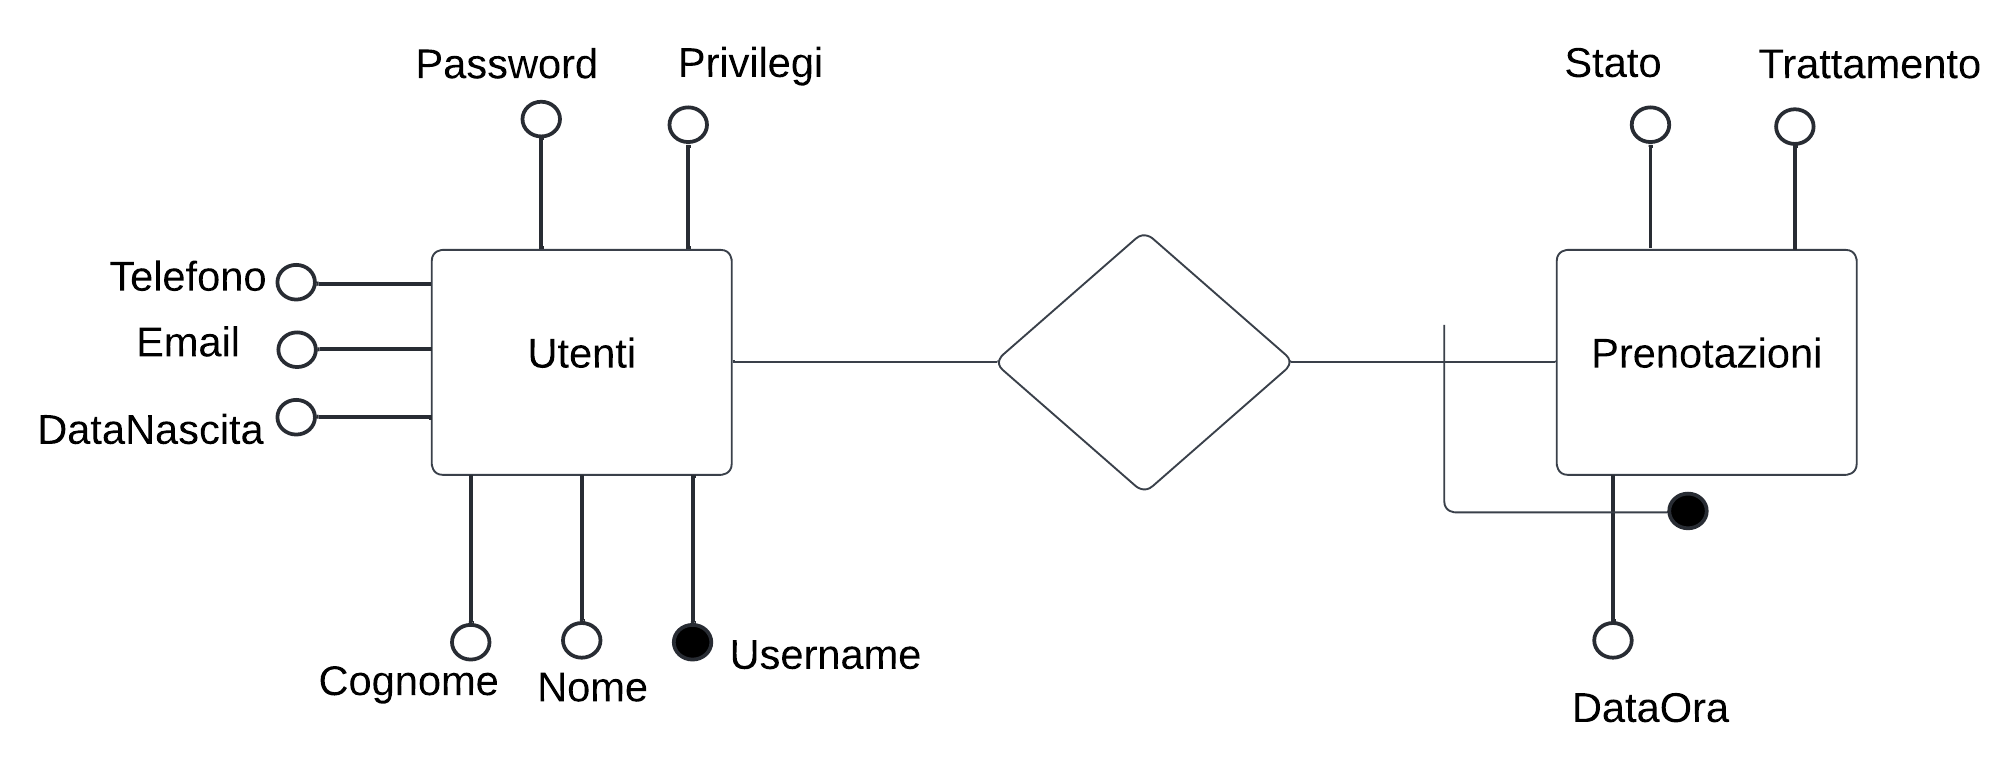
\includegraphics[width=\textwidth]{./graphics/er.png}}
	\caption{Diagramma ER del database}
\end{figure}

Nella parte di analisi si sono elencate tre figure: l'utente generico, l'utente autenticato e l'amministratore.\\
Per permettere questa distinzione, nel database sono inseriti solo i dati degli utenti registrati e dell'amministratore, in modo da poterne determinarne i privilegi, e conseguentemente le pagine visualizzabili o meno.\\
É inoltre necessario l'utilizzo delle due tabelle in quanto le pagine Area Personale e le relative pagine per la prenotazione necessitano di essere create dinamicamente, altrimenti risulterebbero vuote.\\
Quindi, il database é stato progetto in maniera da salvare il numero minimo di informazioni necessarie per una gestione ottimale del sito, mantenendo comunque una predisposizione alla sua evolvibilitá. Se per esempio si volesse inserire un'entitá per rappresentare i trattamenti, ció permetterebbe di effettuare una minuscola modifica alla tabella Prenotazioni, senza intaccarne la funzionalità.


\section{Presentazione}
Il sito permette 4 modalità di visualizzazione:
\begin{itemize}
	\item \textit{Desktop:} per ogni tipo di device, fornisce le regole generali;
	\item \textit{Mobile:} per device mobili aventi dimensioni ridotte;
	\item \textit{Desktop ad alta definizione:} per device che si sviluppano in larghezza;
	\item \textit{Stampa:} per ogni tipo di device, fornisce le regole da applicare quando si desidera stampare o esportare in formato \textit{PDF} una pagina del sito.
\end{itemize}
Il passaggio da una modalità di visualizzazione ad un'altra è stata gestita in modo da dare continuità alla forma dei contenuti.

\subsection{Desktop}
Il foglio di stile per dispositivi desktop definisce in primis la struttura comune a tutte le pagine del sito, la quale consta di:
\begin{itemize}
	\item \textbf{Logo:} è l'immagine di sfondo del titolo della pagina, il quale viene spostato a sinistra in modo da essere comunque leggibile dagli screen-readers senza essere visibile sul display;
	\item \textbf{Breadcrumb:} è la rappresentazione del percorso che l'utente ha compiuto per arrivare ad una determinata pagina;
	\item \textbf{Menù:} fornisce dei collegamenti rapidi a risorse offerte dal sito e ne sono offerte due versioni: una per gli amministratori (in particolare appena entrano nelle pagine di gestione delle prenotazioni) ed una per gli altri utenti;
	\item \textbf{Footer:} contiene tutti le informazioni di contatto al visitatore e gli orari di apertura del centro estetico.
\end{itemize}

\begin{figure}[H]
	\centering
	\fbox{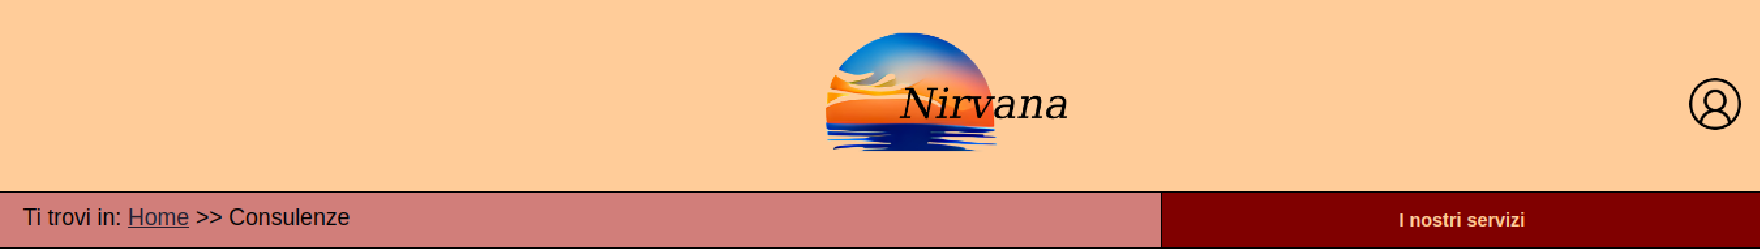
\includegraphics[width=\textwidth]{./graphics/top-common.pdf}}
	\caption{Intestazione delle pagine comprensiva di logo, breadcrumb e menù}
\end{figure}

\begin{figure}[H]
	\centering
	\fbox{
\includegraphics[width=\textwidth]{./graphics/bottom-common.pdf}}
	\caption{Footer delle pagine}
\end{figure}

In questo foglio di stile viene definita anche la struttura grafica specifica per le varie tipologie di pagine presenti nel sito:
\begin{itemize}
	\item \textbf{Pagine semplici:} sono le pagine aventi contenuti prettamente testuali (ad esempio la pagina relativa alle consulenze);
	\item \textbf{Pagine con carte:} il contenuto di tali pagine è composto da riquadri dai bordi arrotondati aventi immagini di sfondo (le "carte" appunto); i riquadri possono essere dei link ad altre pagine oppure possono contenere del testo (ad esempio per spiegare le finalità di alcuni trattamenti);
	\item \textbf{Pagine di gestione:} il contenuto di tali pagine è diviso in due metà costituite da form e/o tabelle relative alla gestione delle prenotazioni.
\end{itemize}

\begin{figure}[H]
	\centering
	\fbox{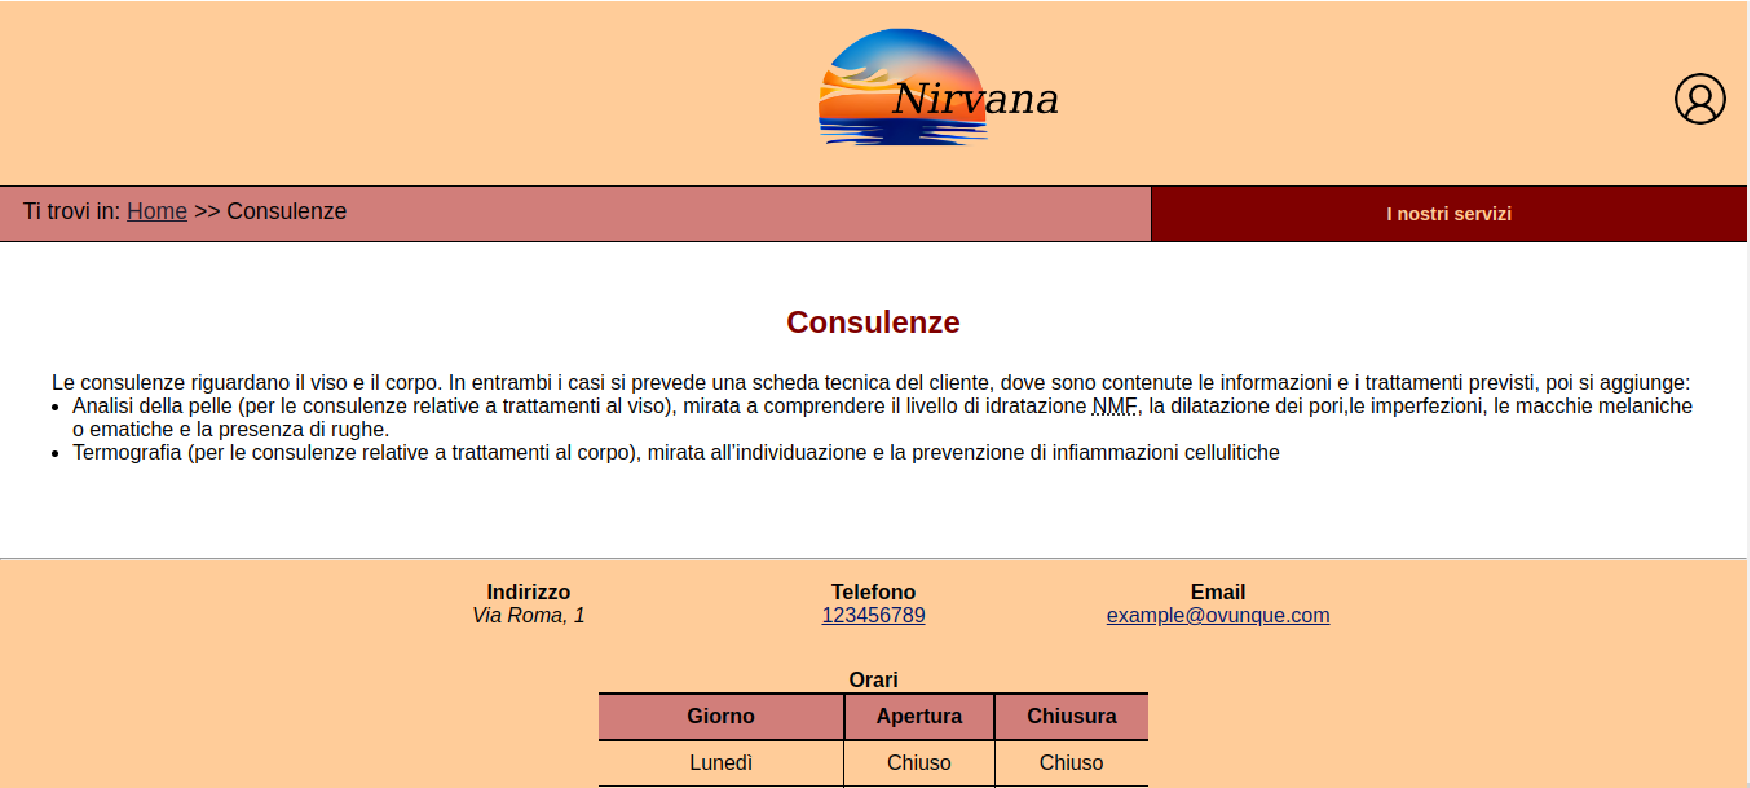
\includegraphics[width=\textwidth]{./graphics/plain-page.pdf}}
	\caption{Pagine semplici}
\end{figure}

\begin{figure}[H]
	\centering
	\fbox{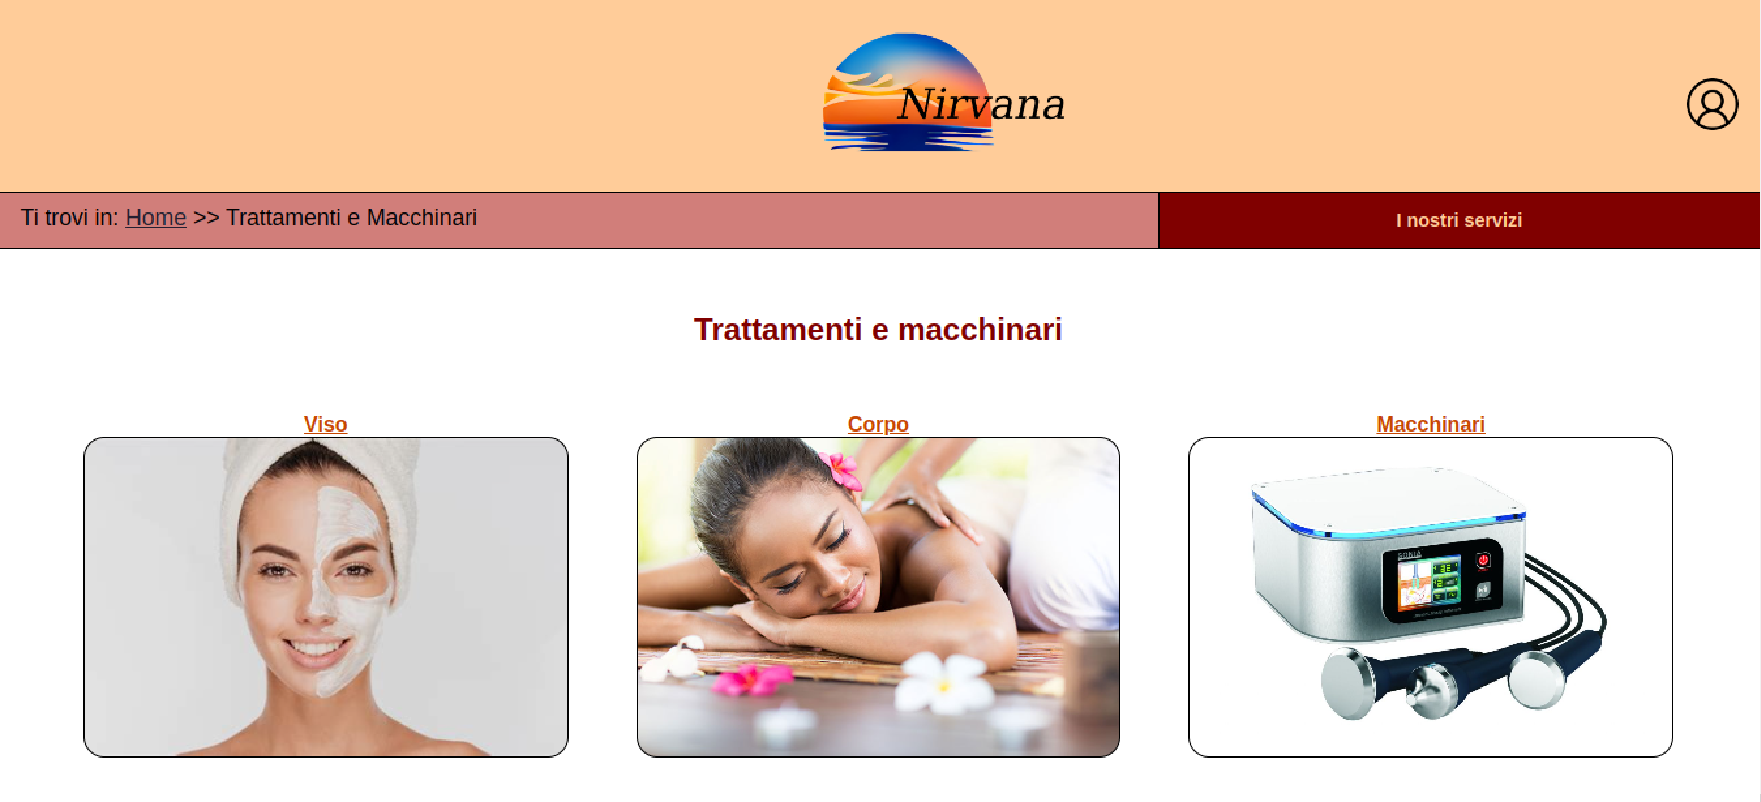
\includegraphics[width=\textwidth]{./graphics/card-page.pdf}}
	\caption{Pagine con carte}
\end{figure}

\begin{figure}[H]
	\centering
	\fbox{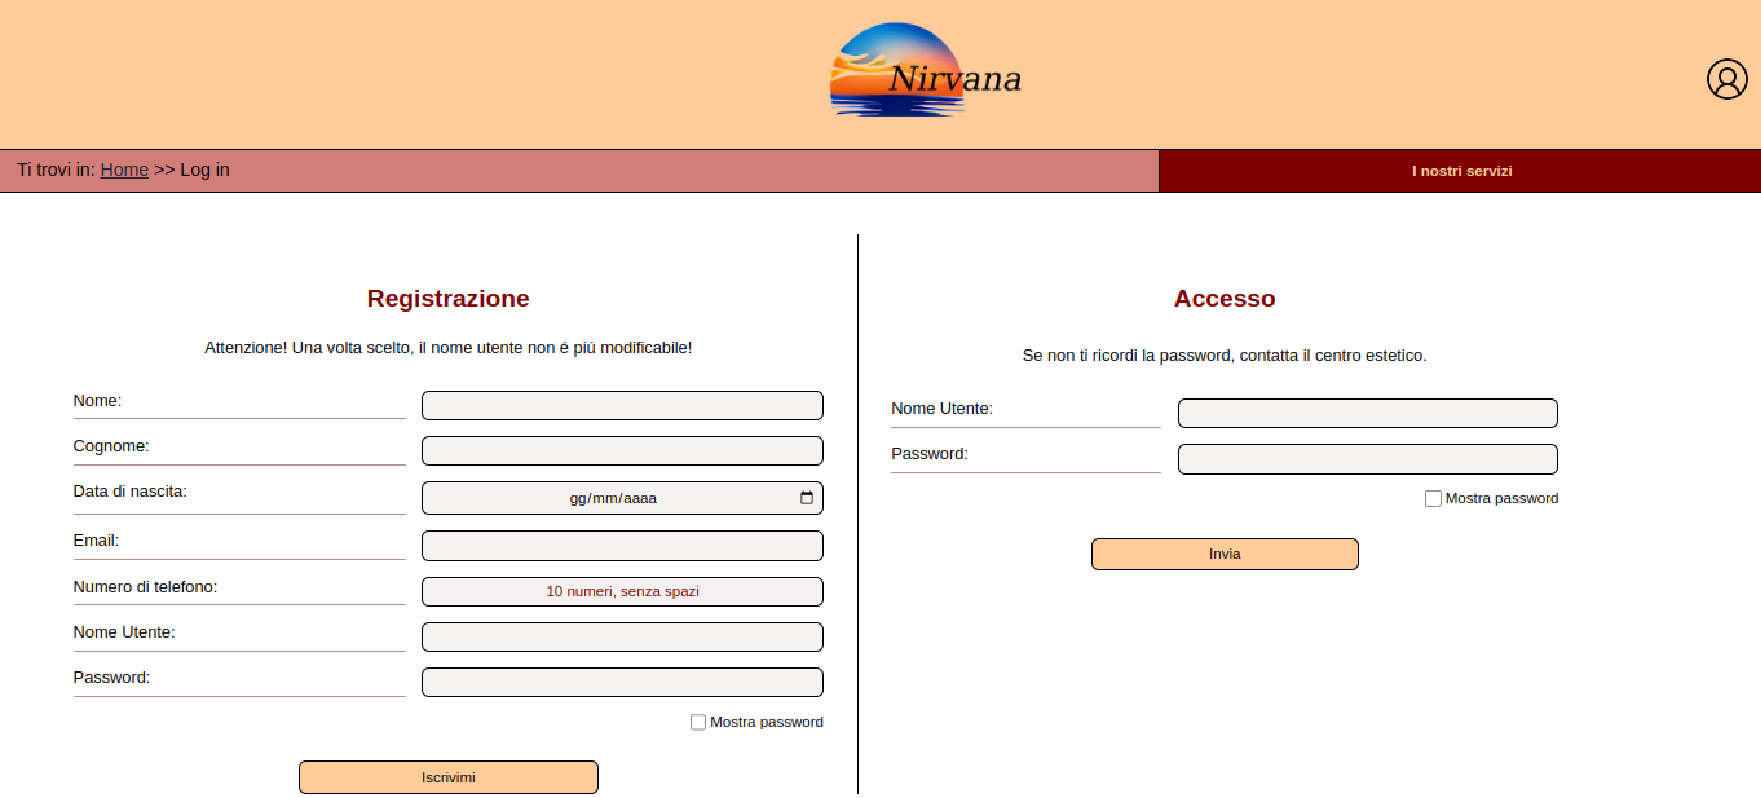
\includegraphics[width=\textwidth]{./graphics/dual-page.pdf}}
	\caption{Pagine di gestione}
\end{figure}

\subsection{Mobile}
\label{presentazione:mobile}
Il foglio di stile relativo a dispositivi mobili viene utilizzato quando la larghezza di schermo offerta per la visualizzazione dei contenuti è inferiore a 1150 pixels: tale misura è stata scelta in modo sperimentale, basandosi inizialmente sulla larghezza della breadcrumb più verbosa.\\
Le principale variazioni di stile riguardano i seguenti elementi:
\begin{itemize}
	\item \textit{Tabelle:} ogni tabella viene convertita in una tabella equivalente avente una sola colonna;
	\item \textit{Grandezza carattere:} viene aumentata la grandezza dei caratteri in modo da migliorare la leggibilità;
	\item \textit{Menù:} il menù utente viene inserito sotto alla breadcrumb, offrendo le stesse funzionalità della versione desktop ma utilizzando in modo più efficiente la larghezza offerta dal dispositivo;
	\item \textit{Bottone utente:} il pulsante relativo alle azioni di login, logout ed accesso all'area personale si scorpora dall'header per rimanere fisso in una zona facilmente raggiungibile da un pollice, "appoggiandosi" sopra al footer quando si arriva a fine pagina.
\end{itemize}
Tramite \textit{media query} che si attiva quando la larghezza a disposizione per la fruizione visiva del sito è inferiore a 940 pixels, alcune breadcrumb particolamente lunghe sono sostituite da breadcrumb aventi riferimento solamente al "livello superiore", ovvero alla pagina che, nella gerarchia di navigazione del sito, si trova immediatamente sopra.
\begin{figure}[H]
	\centering
	\fbox{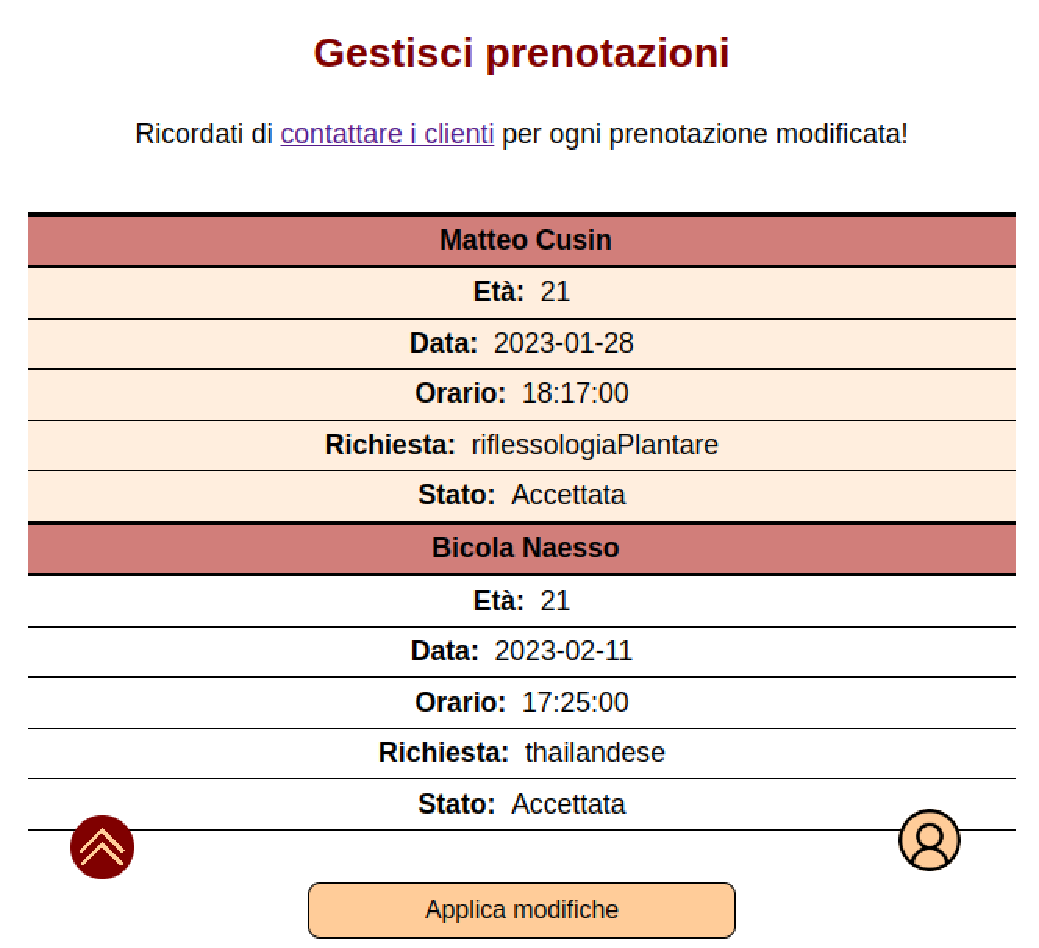
\includegraphics[height=.5\textwidth]{./graphics/table.pdf}}
	\caption{Tabella e bottone}
\end{figure}

\begin{figure}[H]
	\centering
	\fbox{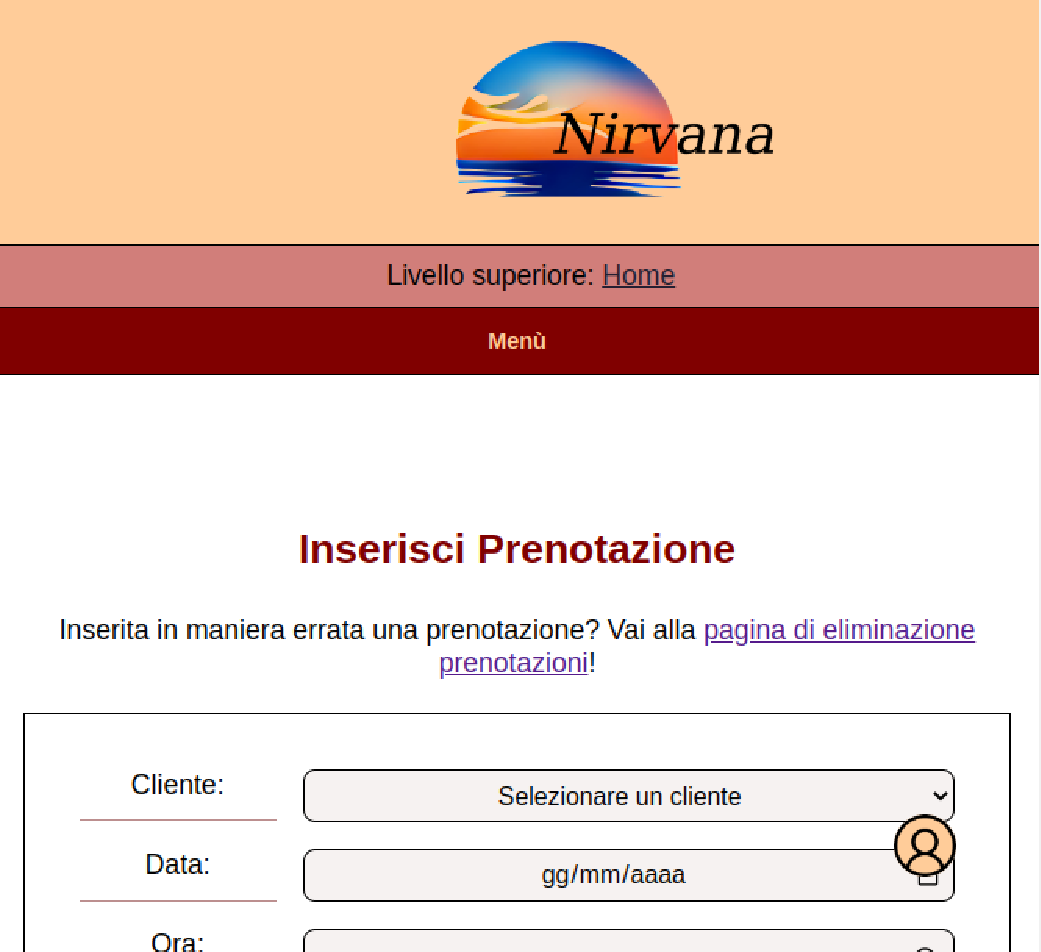
\includegraphics[height=.5\textwidth]{./graphics/menuBreadAndButton.pdf}}
	\caption{Breadcrumb, bottone e menù}
\end{figure}

%TODO Annalisa
\newpage
\subsection{Wide-screen}
Si elencano di seguito le principali variazioni rispetto al corrispondente foglio di stile per desktop generici:
\begin{itemize}
	\item\textit{font-size}: viene incrementato il \textit{font-size} per rendere l'esperienza di navigazione di più immediata leggibilità;
	\item ampiezza del \textit{main}: la sezione \textit{main} è libera di crescere fino ad un massimo di 1500px;
	\item media queries: vengono prese in considerazione specifiche media queries (rispettivamente a 1120px e 1500px), tramite le stesse si hanno effetti collaterali voluti che riprendono lo stile di visualizzazione da mobile.\\
	Si esplicita solo sinteticamente qualche esempio per evitare di essere ridondanti e ripetitivi:  tabelle, bottone utente, utilizzo della \textit{mini-breadcrumb}, etc.; per maggiori dettagli riguardo ai cambiamenti di stile in visualizzazione mobile si rimanda alla sezione \hyperref[presentazione:mobile]{\underline{Mobile}}.
\end{itemize}

\subsection{Print}
Il file relativo alla stampa è stato implementato in modo tale da rimuovere le funzionalità interattive quali link, bottoni, breadcrumb e sezione menù.\\
Per facilitare la leggibilità delle informazioni in modalità cartacea, quelle che nei file .html sono classificate come carte, vengono visualizzate sottoforma di semplice testo.\\
La scelta voluta di non rimuovere il colore di background permette all'utente di scegliere l'opzione "bianco e nero" e "grafica di background" presente in ogni finestra di dialogo stampa dei motori di ricerca favorendo l'esperienza di personalizzazione.\\
Di seguito due  esempi di stampa della stessa pagina:
\begin{figure}[H]
	\centering
	\begin{subfigure}[t]{.5\textwidth}
	  \centering
	  \fbox{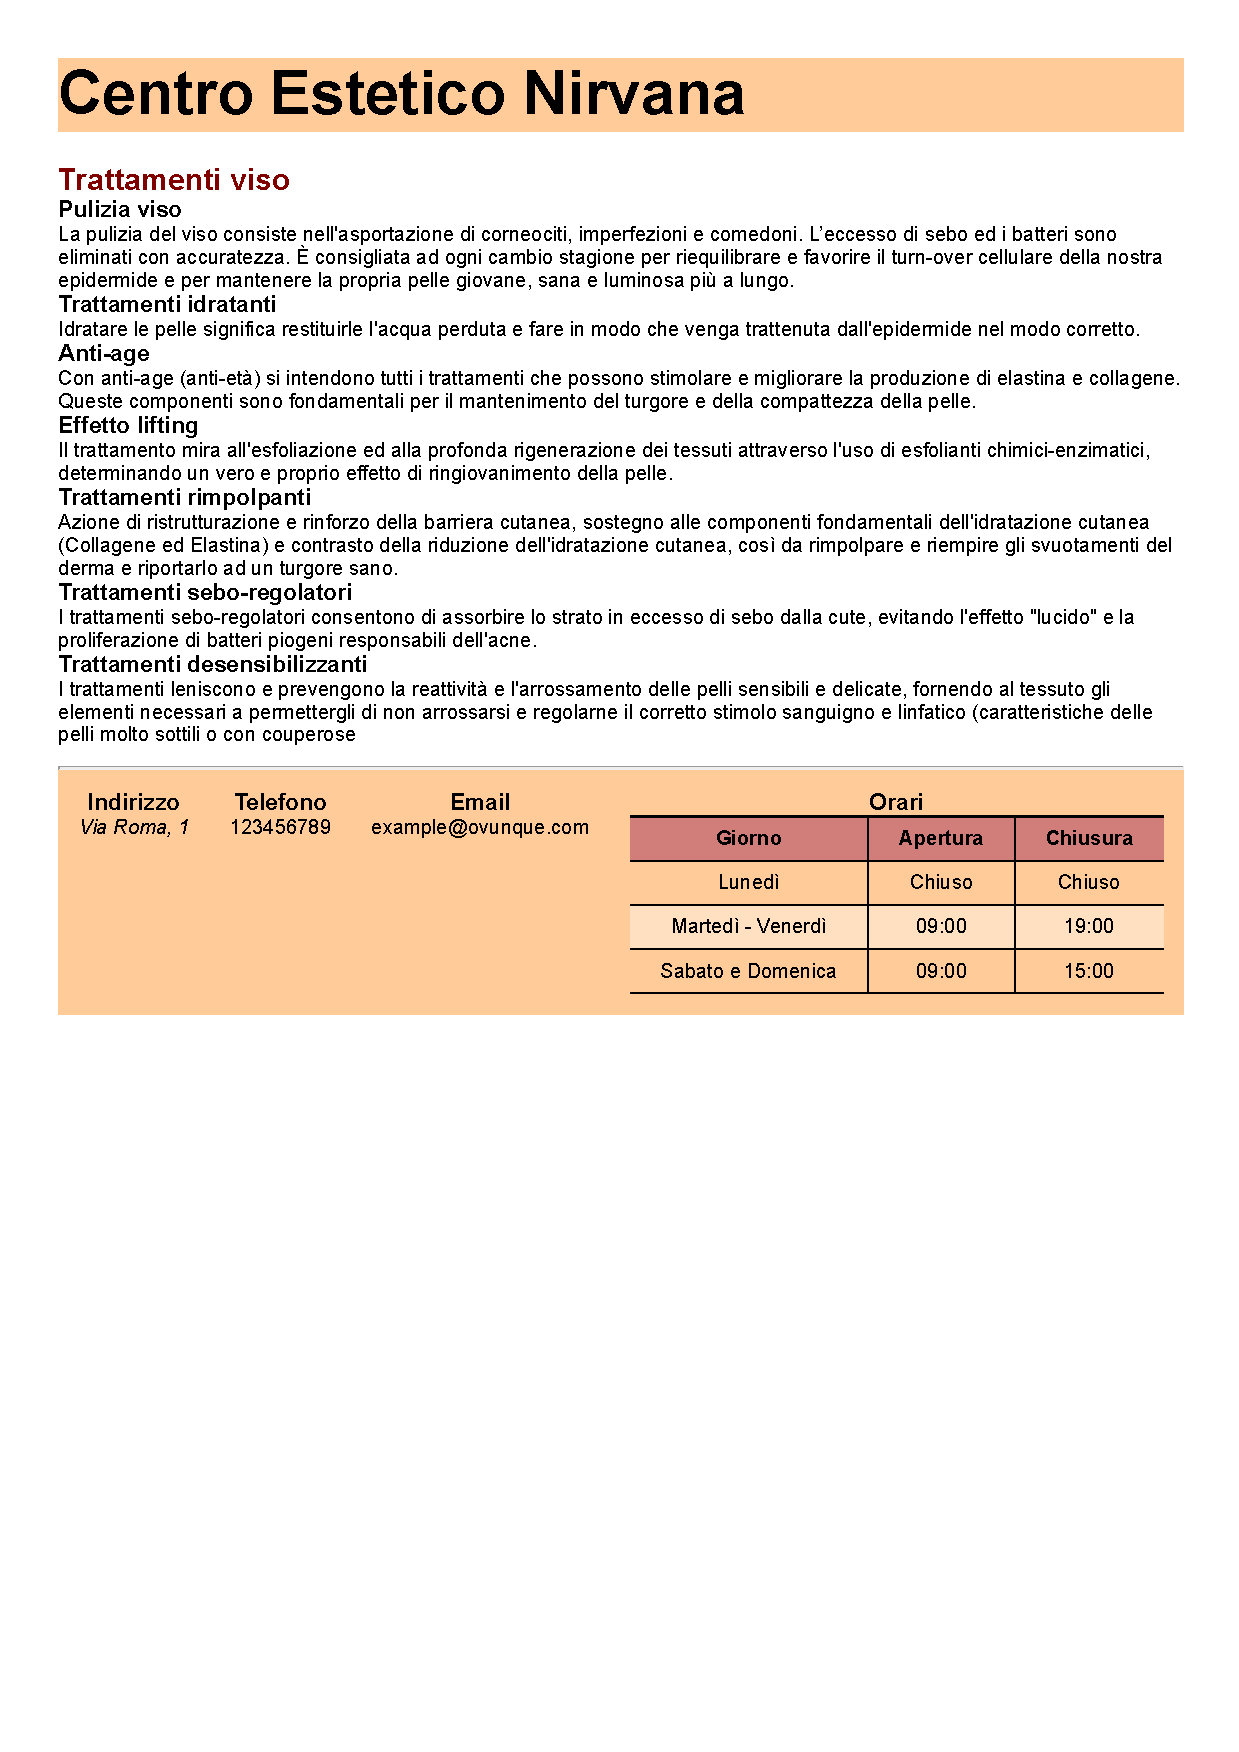
\includegraphics[width=.9\textwidth]{./graphics/NirvanaTrattamentiViso-w.pdf}}
	  \caption{Stampa con colori}
	\end{subfigure}%
	\begin{subfigure}[t]{.5\textwidth}
	  \centering
	  \fbox{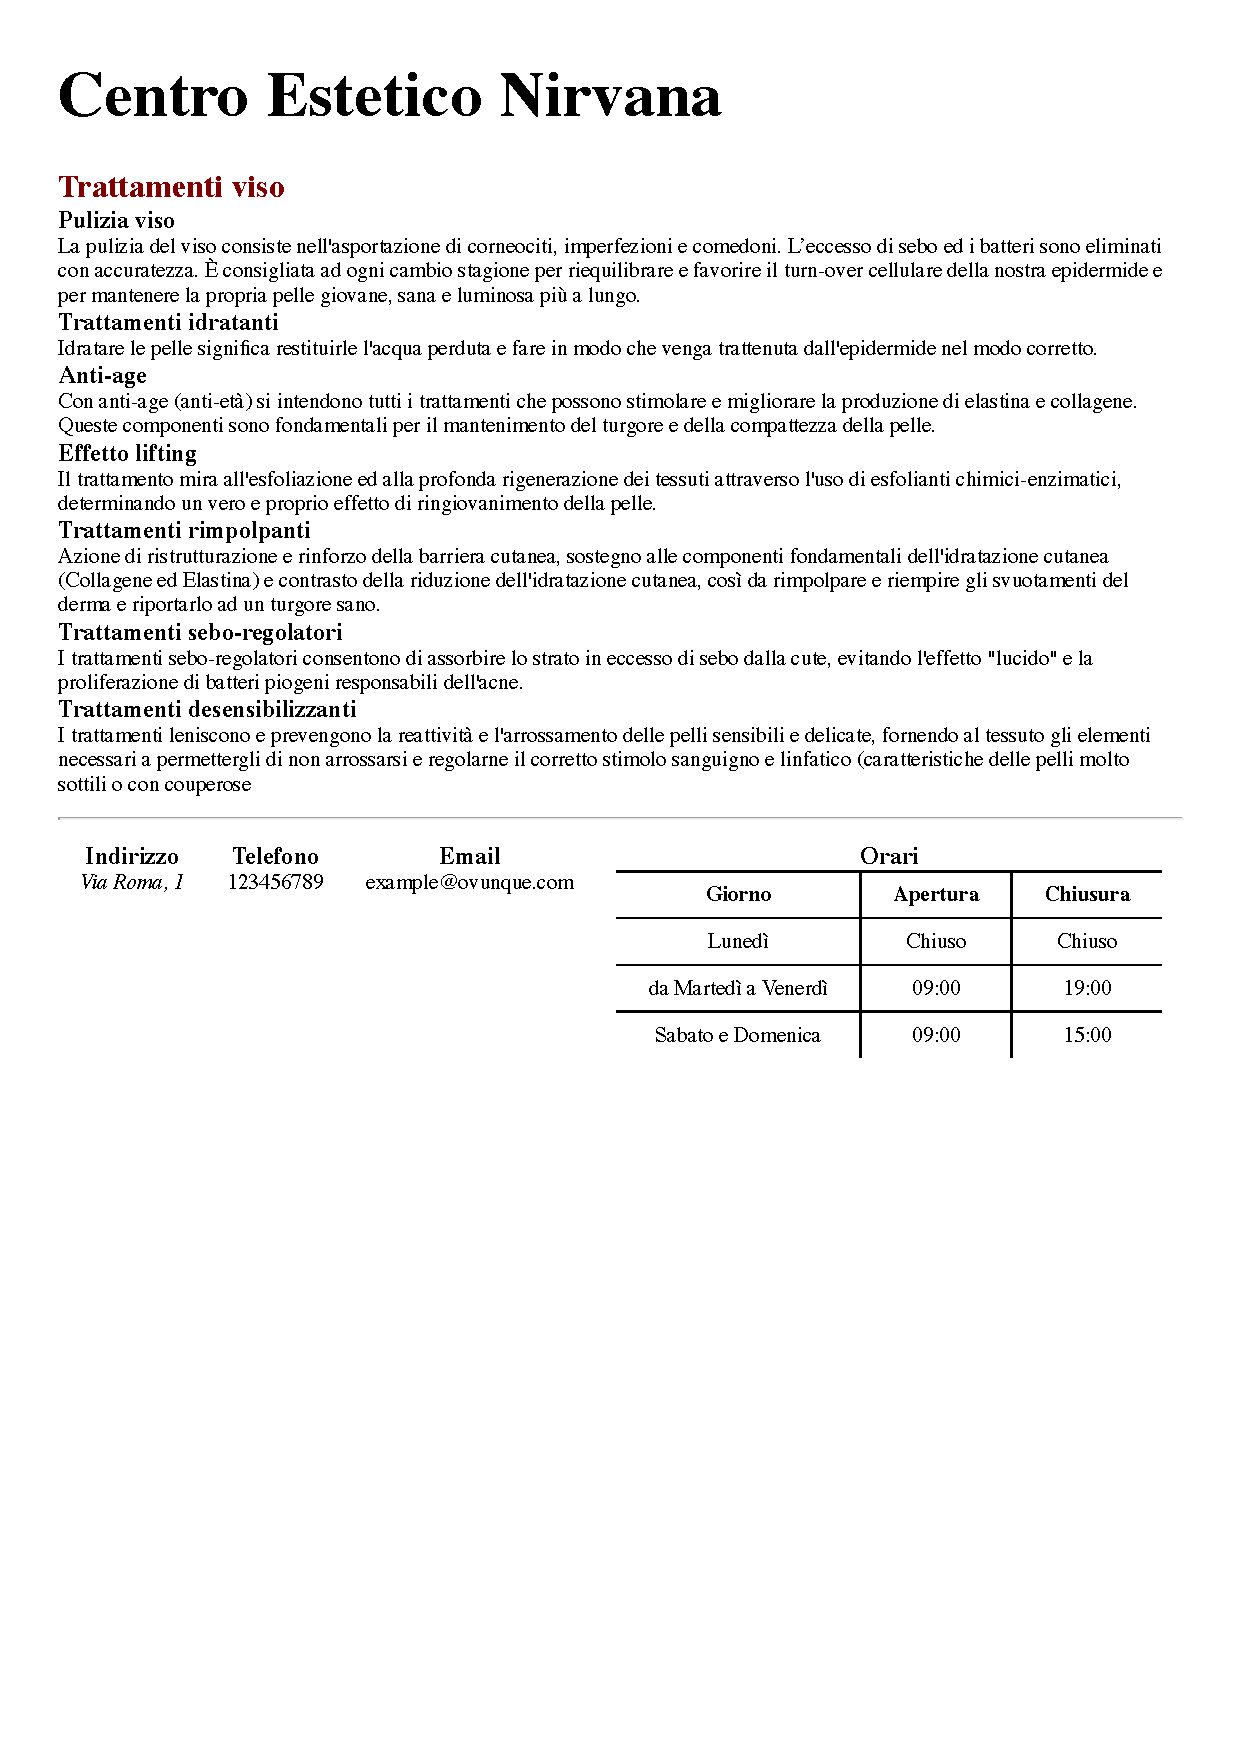
\includegraphics[width=.9\textwidth]{./graphics/NirvanaTrattamentiViso-wo.pdf}}
	  \caption{Stampa senza colori}
	\end{subfigure}
	\caption{Opzioni di stampa}
\end{figure}

%nuova sezione
\section{Implementazione}
\subsection{HTML}
Il progetto è stato realizzato tramite il linguaggio \textit{HTML5} ma si è resa possibile la compatibilità con browser più datati seguendo le linee guida del corso di Tecnologie Web e quelle del \textit{W3C}.
Si è utilizzato \textit{HTML5} piuttosto che \textit{XHTML} in quanto il pubblico cui è destinato il sito web sarà indicativamente di età compresa fra i 16 ed i 60; si presume che la clientela si distribuirà in modo omogeneo in questa fascia d'età, avente quindi a disposizione motori di ricerca tendenzialmente più recenti.\\
I file \textit{.html} si presentano con l'obbiettivo di mantenere struttura, presentazione e contenuto il più possibile separati fra loro.

Per quanto concerne i \textit{tag}:
\begin{itemize}
	\item si sono utilizzati \textit{tag} semantici che arricchiscono il progetto in accessibilità;
	\item si è controllata la chiusura di tutti i \textit{tag};
	\item i \textit{metatag} presenti nella sezione \textit{head} dei file \textit{.html} aiutano il sito nel ranking di ricerca e sono di fondamentale importanza per incrementare l'accessibilità.
\end{itemize}

\subsection{CSS}
La modellazione del layout del sito è stata implementata tramite CSS3.\\
Per rendere l'esperienza di navigazione fluida tra i vari dispositivi, sono state utilizzate misure relative ed in percentuale.\\
Abbiamo creato 4 fogli di stile per implementare il layout secondo lo specifico ambito d'uso:
\begin{itemize}
	\item \textit{style.css}: foglio di stile predefinito;
	\item \textit{mobile.css}: viene utilizzato dai browser nella condizione in cui lo schermo/spazio di visualizzazione abbia larghezza inferiore a 1150px;
	\item \textit{wide-screen.css}: viene utilizzato dai browser nella condizione in cui lo schermo/spazio di visualizzazione abbia larghezza superiore a 1900px;
	\item \textit{print.css}: viene presa in considerazione all'atto di stampa delle pagine del sito.
\end{itemize}
All'interno dei \textit{.css} prodotti è possibile trovare quantopiù offerto dal \textit{CSS3}, come per esempio: flexbox, grid, media queries, variabili, selettori, etc.\\
Grazie ad alcune accortezze, tramite flexbox, è stata possibile l'implementazione di un layout  "a carte" accattivante che non compromettesse l'accessibilità.

\subsection{PHP} % Matteo e Nicola
Il linguaggio PHP è stato utilizzato per lo sviluppo della parte di comportamento server-side del sito web. \\
La versione del linguaggio scelta dal gruppo è la 8.1 dato che la versione 8.0 non è più supportata dal giorno 26 Novembre 2022 (fino al 26 Novembre 2023 saranno effettuati aggiornamenti puramente relativi alla sicurezza).
\begin{figure}[H]
	\centering
	\fbox{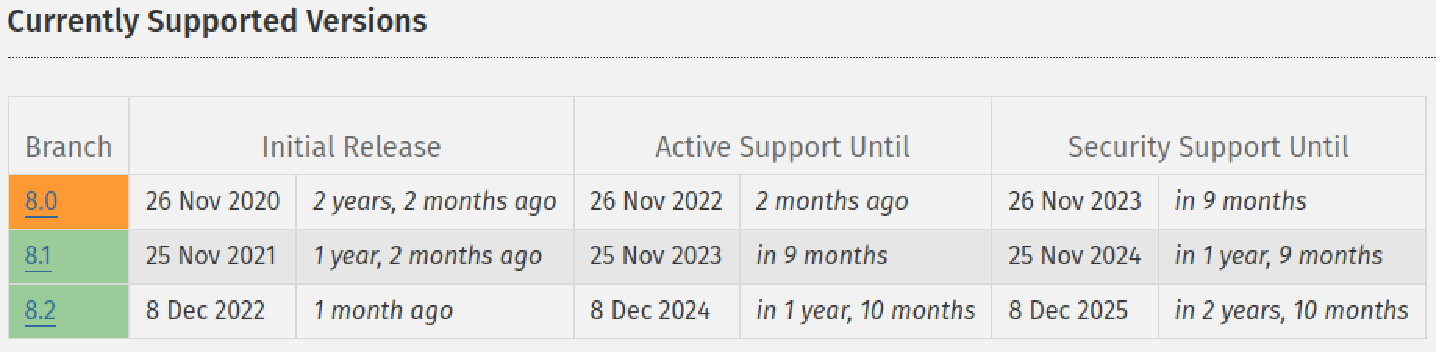
\includegraphics[width=\textwidth]{./graphics/php-support.pdf}}
	\caption{\href{https://www.php.net/supported-versions.php}{https://www.php.net/supported-versions.php} al 30 Gennaio 2023}
\end{figure}

\subsubsection{Autenticazione}
\paragraph*{Login}
\paragraph*{Logout}

\subsubsection{Connessione}

\subsubsection{Area personale}
\paragraph*{Area personale}
\paragraph*{Elenco clienti}

\subsubsection{Prenotazioni}
\label{prenotazioni:valida}
Con il termine \textbf{\textit{prenotazione valida}} utilizzato nei paragrafi seguenti si intende una prenotazione avente data-ora \textit{posteriore} rispetto alla data-ora in cui la prenotazione è presa in analisi: se un utente registrato vuole richiedere una prenotazione, essa deve essere valida e, per essere valida, deve avere data-ora \textit{successiva} alla data-ora in cui avviene la richiesta di prenotazione.

\paragraph*{Gestione prenotazioni lato utente}
La pagina di gestione delle prenotazioni, per l'utente registrato, si divide in due parti:
\begin{itemize}
	\item Richiesta di prenotazione;
	\item Visualizzazione delle richieste di prenotazione.
\end{itemize}
La richiesta di una prenotazione consiste nell'aggiungere una prenotazione \hyperref[prenotazioni:valida]{\underline{valida}} alla base di dati con stato "In fase di approvazione": un utente con privilegi di \textit{amministrazione} dovrà occuparsi di accettare o rifiutare la prenotazione e tale cambiamento di stato sarà visualizzabile dall'utente registrato nella relativa tabella.
\begin{figure}[H]
	\centering
	\fbox{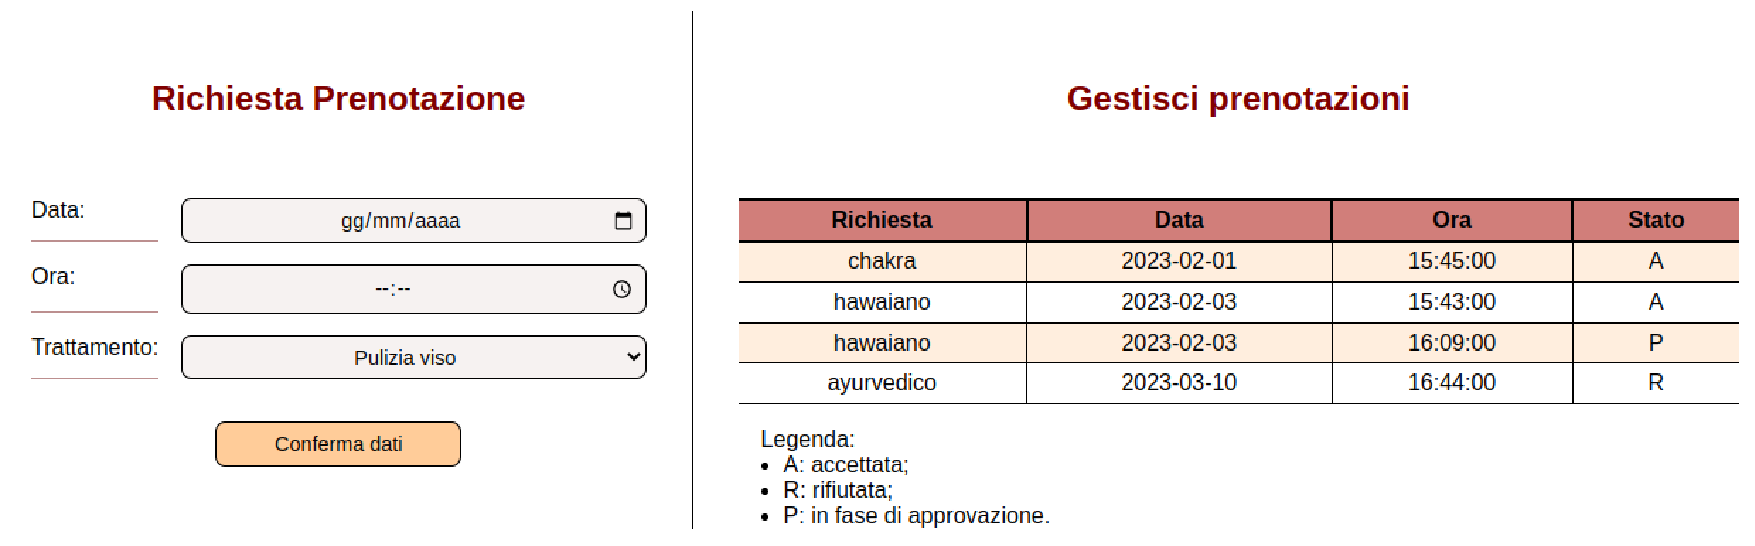
\includegraphics[width=\textwidth]{./graphics/userReservations.pdf}}
	\caption{Pagina di gestione prenotazioni utente}
\end{figure}

\paragraph*{Gestione prenotazioni lato amministratore}
La pagina di gestione delle prenotazioni, per l'utente amministratore, si divide in due parti:
\begin{itemize}
	\item Inserimento di prenotazioni;
	\item Gestione delle richieste di prenotazione.
\end{itemize}
L'inserimento di una prenotazione consiste nell'aggiungere una prenotazione \hyperref[prenotazioni:valida]{\underline{valida}} alla base di dati con stato "accettato" per un utente registrato: questo è fatto in quanto la fase di approvazione è inclusa nella fase di richiesta della prenotazione se viene effettuata da un amministratore (che dovrebbe altrimenti approvare la propria richiesta di prenotazione).
\begin{figure}[H]
	\centering
	\fbox{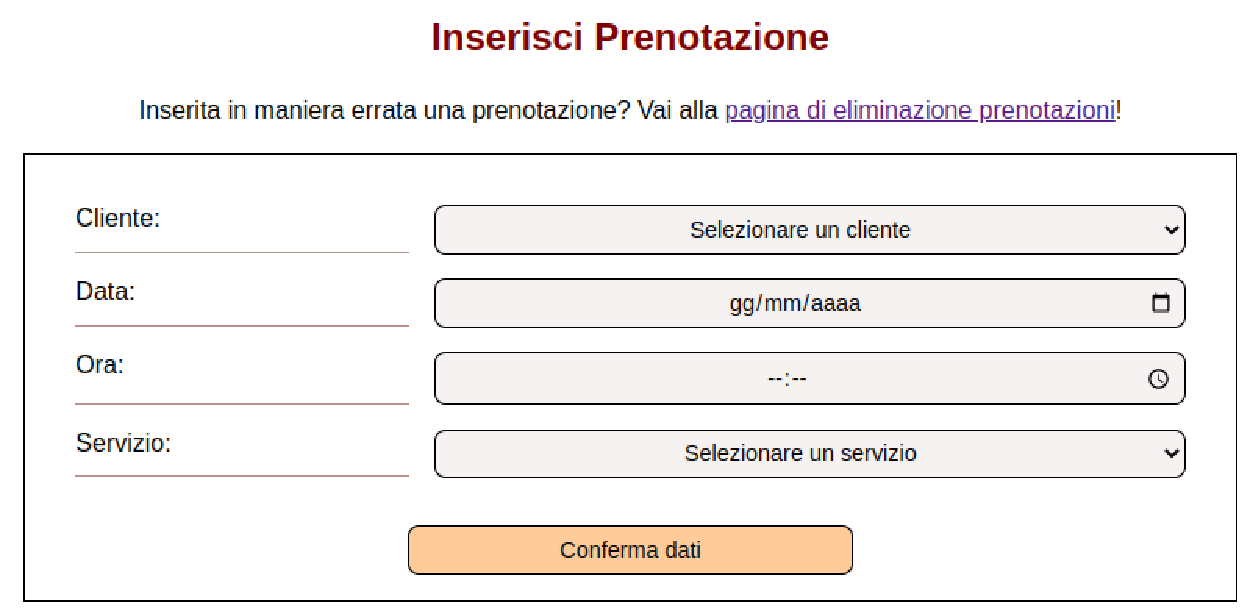
\includegraphics[width=\textwidth]{./graphics/insertReservations.pdf}}
	\caption{Inserimento prenotazioni lato amministrativo}
\end{figure}
La conferma o meno di una prenotazione avviene tramite un form organizzato in forma tabellare dal quale l'amministratore può anche modificare la data-ora della richiesta (si pensi a situazioni di richieste multiple sovrapposte temporalmente).
\begin{figure}[H]
	\centering
	\fbox{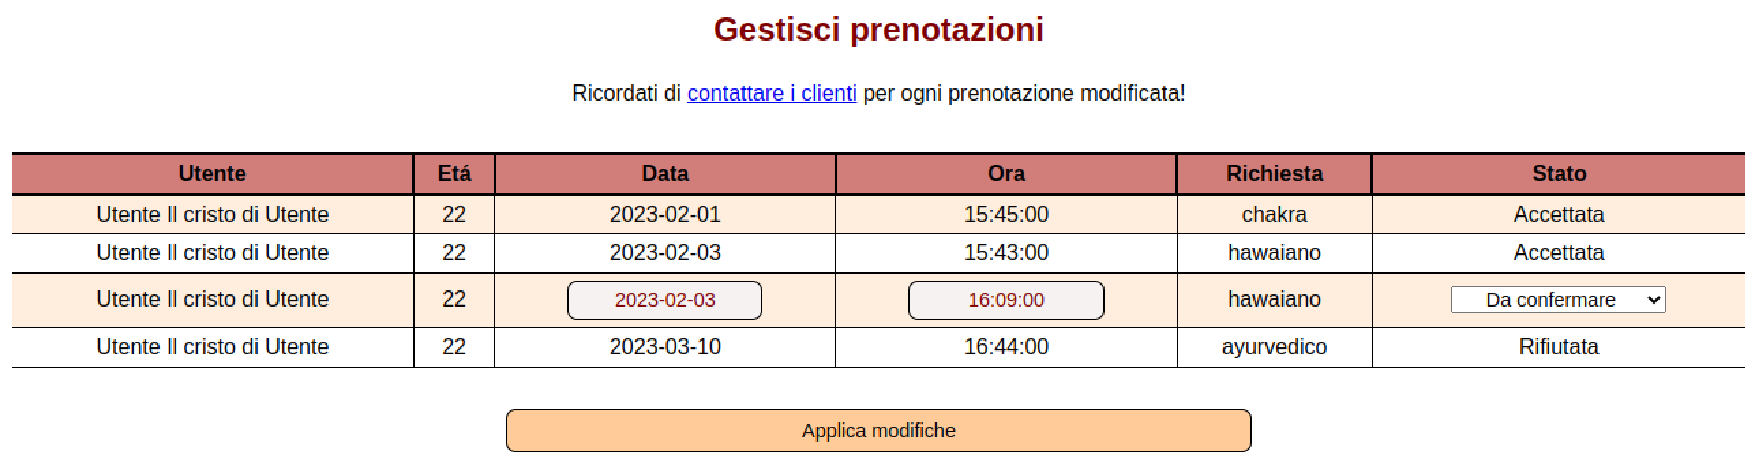
\includegraphics[width=\textwidth]{./graphics/adminReservations.pdf}}
	\caption{Gestione prenotazioni lato amministrativo}
\end{figure}

\paragraph*{Eliminazione prenotazioni}
Si è deciso di separare l'operazione di eliminazione delle prenotazioni dalla pagina di \textit{Gestione delle prenotazioni lato amministratore} per dividere le operazioni \textbf{CRUD} in più pagine, evitando un sovraccarico cognitivo da parte dell'utente amministratore (dovuto alla presenza di troppe informazioni in un'unica pagina). \\
La logica seguita dalla pagina è la seguente: l'amministratore ha la possibilità di visualizzare ogni prenotazione considerata \hyperref[prenotazioni:valida]{\underline{valida}} tramite una tabella e può eseguire un'\textit{eliminazione multipla} selezionando una \textbf{checkbox} che si trova nella stessa riga della tabella della prenotazione da eliminare. \\

\begin{figure}[H]
	\centering
	\fbox{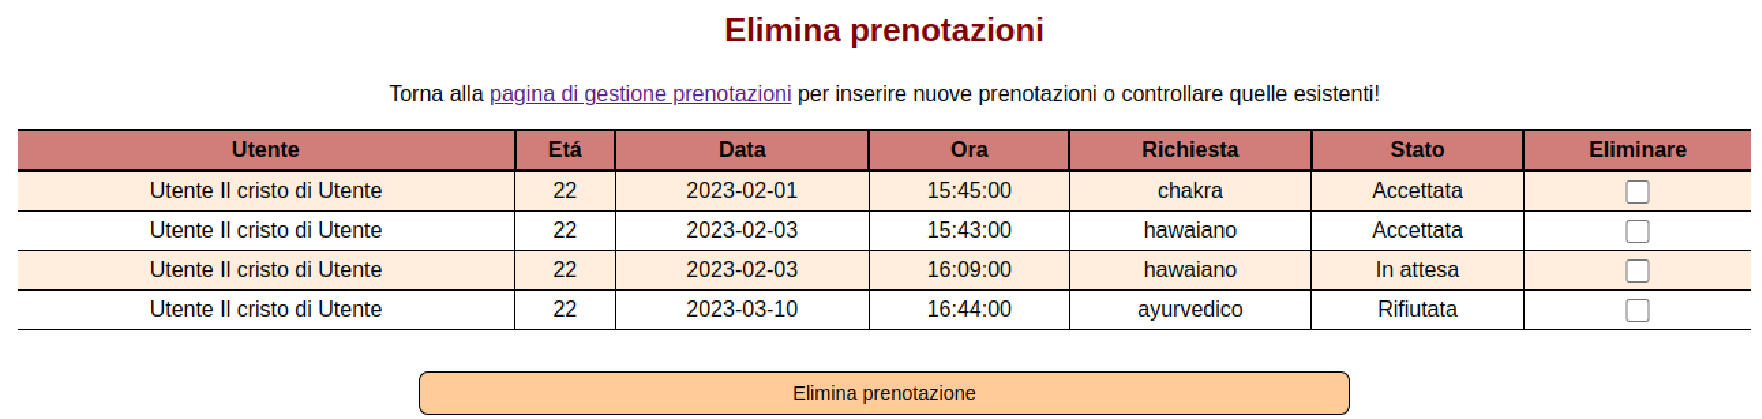
\includegraphics[width=\textwidth]{./graphics/delete.pdf}}
	\caption{Tabella di eliminazione prenotazioni}
\end{figure}

Ogni checkbox ha, come valore associato, la tripla \textbf{Nome Utente}, \textbf{Data di prenotazione} e \textbf{Orario di prenotazione} ed essa costituisce l'identificativo di ogni prenotazione (vedi sottosezione \hyperref[subsec:database]{\underline{database}}); il valore delle checkboxes viene recuperato tramite apposita funzione \textit{PHP} ed è usato per eliminare la relativa prenotazione.

\subsubsection{Amministrazione}
\paragraph*{Errore 401}
\paragraph*{Errore 403}
\paragraph*{Errore 404}
\paragraph*{Errore 500}
\subsection{SQL}	% Nicola
\subsection{JavaScript} %Lisien
\textit{JavaScript} é un linguaggio che viene eseguito dal lato utente, tramite il browser; è utilizzato per dare un determinato comportamento ai siti web tramite l'invocazione di funzioni in seguito all'occorrenza di eventi.\\
Nel sito é usato per cambiare dinamicamente le classi degli elementi HTML ed il tipo di input nei vari form e tabelle.\\
Nei seguenti elementi vengono modificate le classi (per assegnare uno stile particolare in base alla situazione) con l'uso delle funzioni \textit{toggle}, \textit{add}, o \textit{remove} presenti nel linguaggio JavaScript:
\begin{itemize}
        \item \textit{Menú:} se il menú viene cliccato, le sue voci compaiano o scompaiono a seconda dello stato logico del menù (aperto o chiuso); tale funzionalità è stata implementata utilizzando la funzione \textit{toggle};
        \item \textit{Menú personale:} ad ogni caricamento della pagina, una funzione JavaScript controlla se é stato effettuato il login o meno e, in base a questo, viene visualizzata la voce \textbf{login} o \textbf{logout} (sono mutualmente esclusive).
\end{itemize}
Nel progetto sono stati utilizzati i seguenti eventi tramite JavaScript:
\begin{itemize}
        \item \textit{Click:} all'evento "click", se il menù è nello stato \textit{aperto}, questa funzione semplicemente toglie le classi che fanno comparire le voci di menú;
        \item \textit{Scroll:} all'evento "scroll" verso l'alto, compare un'icona rossa con posizione fissa (in una zona facilmente raggiungibile anche da mobile) che consente di spostare la visualizzazione verso la cima della pagina in modo controllato (\textbf{smooth}) tramite un'altra funzione JavaScript.
\end{itemize}
Altre funzioni scritte in JavaScript sono state ideate per device mobili, per facilitare al utente l'accesso al menù personale:
\begin{itemize}
        \item \textit{Menú personale:} questa funzione consente al bottone che rappresenta il menù personale nella visualizzazione mobile di "fermare" la sua discesa (in seguito a \textit{scroll} verso il basso) immediatamente sopra al footer della pagina (come se si "appoggiasse").
\end{itemize}
Vi sono infine altre funzioni che si occupano di cambiare il valore dell'attributo "type" degli elementi HTML "input":
\begin{itemize}
        \item \textit{Mostra password:} questa funzione viene utilizzata tramite checkbox associata ad una casella di testo atta a contenere password; come si evince dal nome, consente di visualizzare in chiaro il valore inserito in tale casella di testo;
        \item \textit{MakeDate, MakeTime:} tali funzioni sono applicate sulla tabella di gestione delle prenotazioni lato amministratore e nell'area personale, rispettivamente al cambio della data o dell'ora delle prenotazioni non accettate ed al cambio dei dati personali.
\end{itemize}
 
%nuova sezione
\section{Validazione}

%nuova sezione
\section{Fase di Test}

%nuova sezione
\section{Strumenti}
A supporto dello sviluppatore, é necessario che siano presenti degli strumenti per guidarlo in uno sviluppo efficiente e in un testing accurato.\\
Vengono sottolineate due categorie di strumenti poiché alcuni strumenti utilizzati non sono adatti per una fase di test, ma risultano estremamente utili come aiuto allo sviluppo.
\subsection{Strumenti di sviluppo}
\subsection{Strumenti di test}
\section{Suddivisione del lavoro}
Per garantire una buona suddivisione del carico di lavoro che il progetto ha inevitabilmente richiesto, si é suddiviso il lavoro tra i membri del gruppo in questo modo:
\begin{itemize}
	\item Lisien Skenderi: 
	\begin{itemize}
		\item HTML: sviluppo delle seguenti pagine: Index, Consulenze, Gestione Prenotazioni - Cliente;
		\item CSS:  elaborazione coordinata del file style.css con particolare attenzione alle sezioni header, breadcrumb e le altre navigazione;
		\item Javascript: sviluppo delle funzioni per il menú principale, il menú utente ed il bottone per l'auto-scroll;
		\item PHP: backend relativo al prenotazione utente, e realizzazione della pagina di logout;
		\item Immagini: acquisizione immagini di sfondo per i bottoni;
		\item Relazione: sottosezione JavaScript.
	\end{itemize}
	\item Matteo Cusin:
	\begin{itemize}
		\item HTML: sviluppo delle seguenti pagine: Trattamenti Viso, Login e Registrazione, Eliminazione prenotazioni;
		\item CSS: creazione e sviluppo di mobile.css, elaborazione coordinata del file style.css con particolare attenzione alle sezioni footer e main;
		\item Javascript: funzione per mostrare in chiaro la password;
		\item PHP: backend relativo all'eliminazione delle prenotazioni;
		\item Immagini: compressione delle immagini utilizzate ed eliminazione delle immagini non utilizzate;
		\item Relazione: sezione progettazione (senza la sottosezione \textit{database}), sviluppo condiviso sezione presentazione desktop, sviluppo sezione presentazione mobile.
	\end{itemize} 
	\item Annalisa Egidi:
	\begin{itemize}
		\item HTML: sviluppo coordinato delle seguenti pagine: 404, areaPersonale, file di trattamenti e index /**/;
		\item CSS: creazione e sviluppo di print.css, elaborazione coordinata del file style.css con particolare attenzione alle sezioni footer e main;
		\item Javascript: funzione per mostrare in chiaro la password;
		\item PHP: /**/
		\item Immagini: ricerca e modifica coordinata delle immagini, implementazione codice per l'utilizzo delle stesse;
		\item Relazione: sezione progettazione, sviluppo condiviso sezione presentazione desktop, sottosezione relativa al foglio di stile per la stampa. 
	\end{itemize} 
	\item Nicola Baesso:
	\begin{itemize}
		\item HTML: sviluppo delle seguenti pagine: ;
		\item CSS:
		\item Javascript:
		\item PHP: backend dei form di login e registrazione, backend prenotazioni lato amministratore e cliente;
		\item Immagini:
		\item Relazione:
	\end{itemize} 
\end{itemize}

\end{document}